% vim: expandtab softtabstop=2 shiftwidth=2 foldmethod=marker spell

\section{Turning the songbot on and off}
For small communities where the chat moves slowly, the best practice for turning the songbot on and off is to use the chat command \lstinline{!setrequests on/off}. This lets the streamer see that the bot is turned on or off. There is also a shortcut for the command \lstinline{!srs on/off}. It is important to note that mods can add songs when requests are off.

\begin{figure}[ht!]
  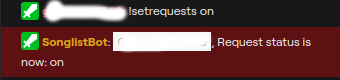
\includegraphics[width=\linewidth]{src/songbot_on_off/setrequests_on.png}
  \caption{The chat messages to turn on the songbot}
  \label{setrequests on}
\end{figure}
\begin{figure}[ht!]
  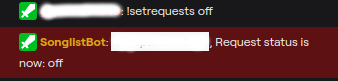
\includegraphics[width=\linewidth]{src/songbot_on_off/setrequests_off.png}
  \caption{The chat messages to turn off the songbot}
  \label{setrequests off}
\end{figure}
\newpage

An alternative to the chat commands is to use the web interface of \mbox{streamersonglist}.
\begin{figure}[ht!]
  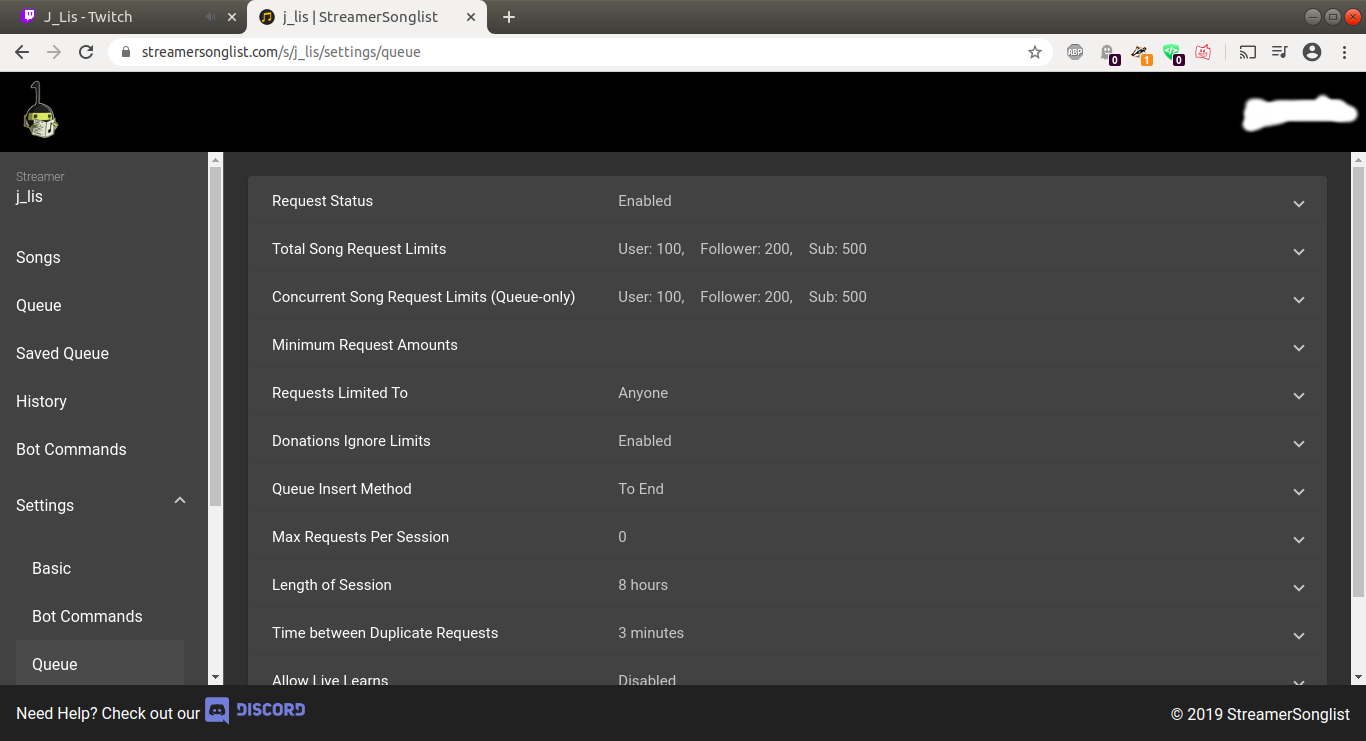
\includegraphics[width=\linewidth]{src/songbot_on_off/bot_on.png}
  \caption{The webpage with the songbot turned on}
  \label{bot is on}
\end{figure}
\begin{figure}[ht!]
  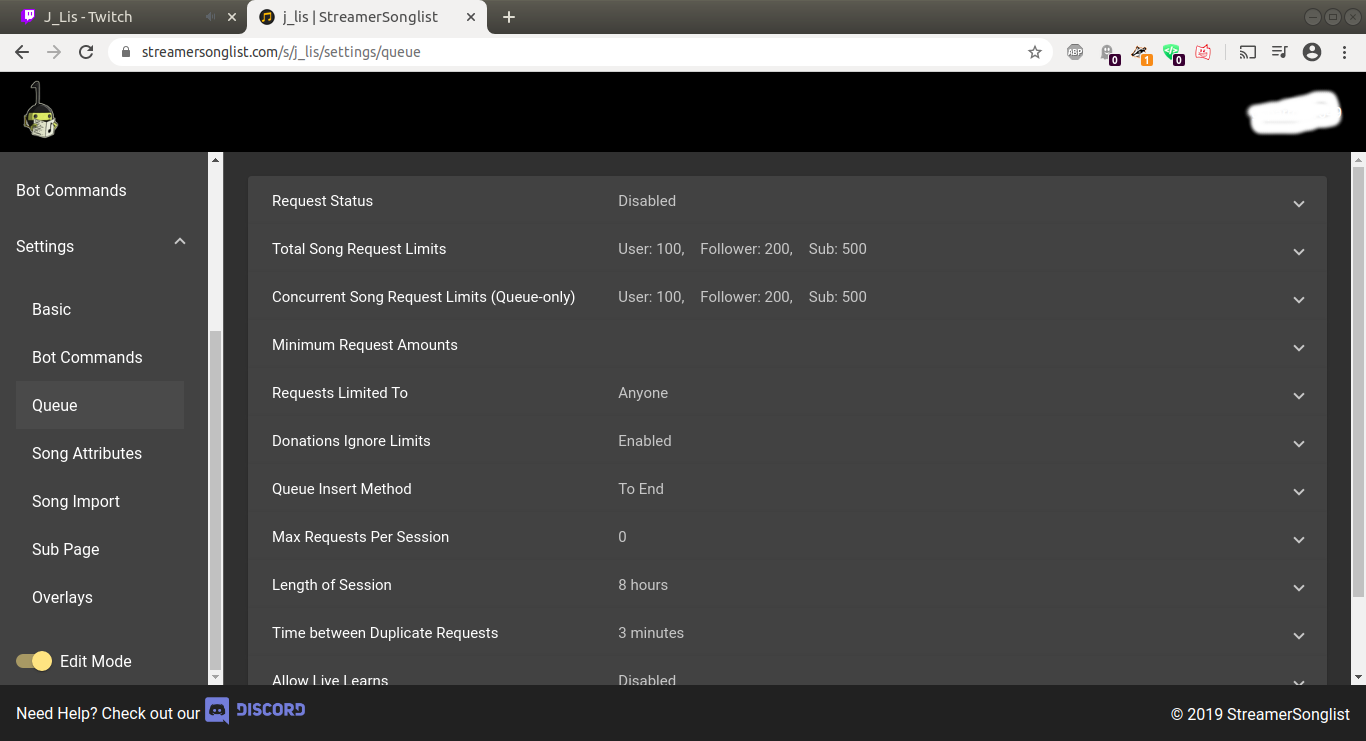
\includegraphics[width=\linewidth]{src/songbot_on_off/bot_off.png}
  \caption{The webpage with the songbot turned off}
  \label{bot is off}
\end{figure}

